\chapter{Research Problem} \label{chap:problem}

This chapter intends to clarify the problem addressed by the present dissertation. Section \ref{sec:prob-state} presents the details behind the research work as well as the problems it intends to solve. Having this clear, the dissertation hypothesis is stated in section \ref{sec:hypoth-rq} along with the research questions that are the main issues that are being explained with the present document. Lastly, the used validation methods are specified in section \ref{sec:validation}.

%------------------------------------------------------------------------------------
\section{Problem Statement} \label{sec:prob-state}

The Ultra-Short Baseline system is among the most deployed positioning methods using underwater acoustics. There is a vast knowledge of its function and capabilities, therefore its implementation does not constitute a technological innovation nowadays. 
In the considered scenario, previously mentioned in chapter \ref{chap:intro}, an AUV is taking part on a long-term underwater mission in which it periodically sends known signals to the surface with a pinger. In such case, the mule AUV needs to be provided with an USBL system to receive the signal and estimate the position of the other AUV to navigate near it. The simplified communication system is illustrated in figure \ref{fig:grow}. 

\begin{figure}[!htbp]
	\centering
	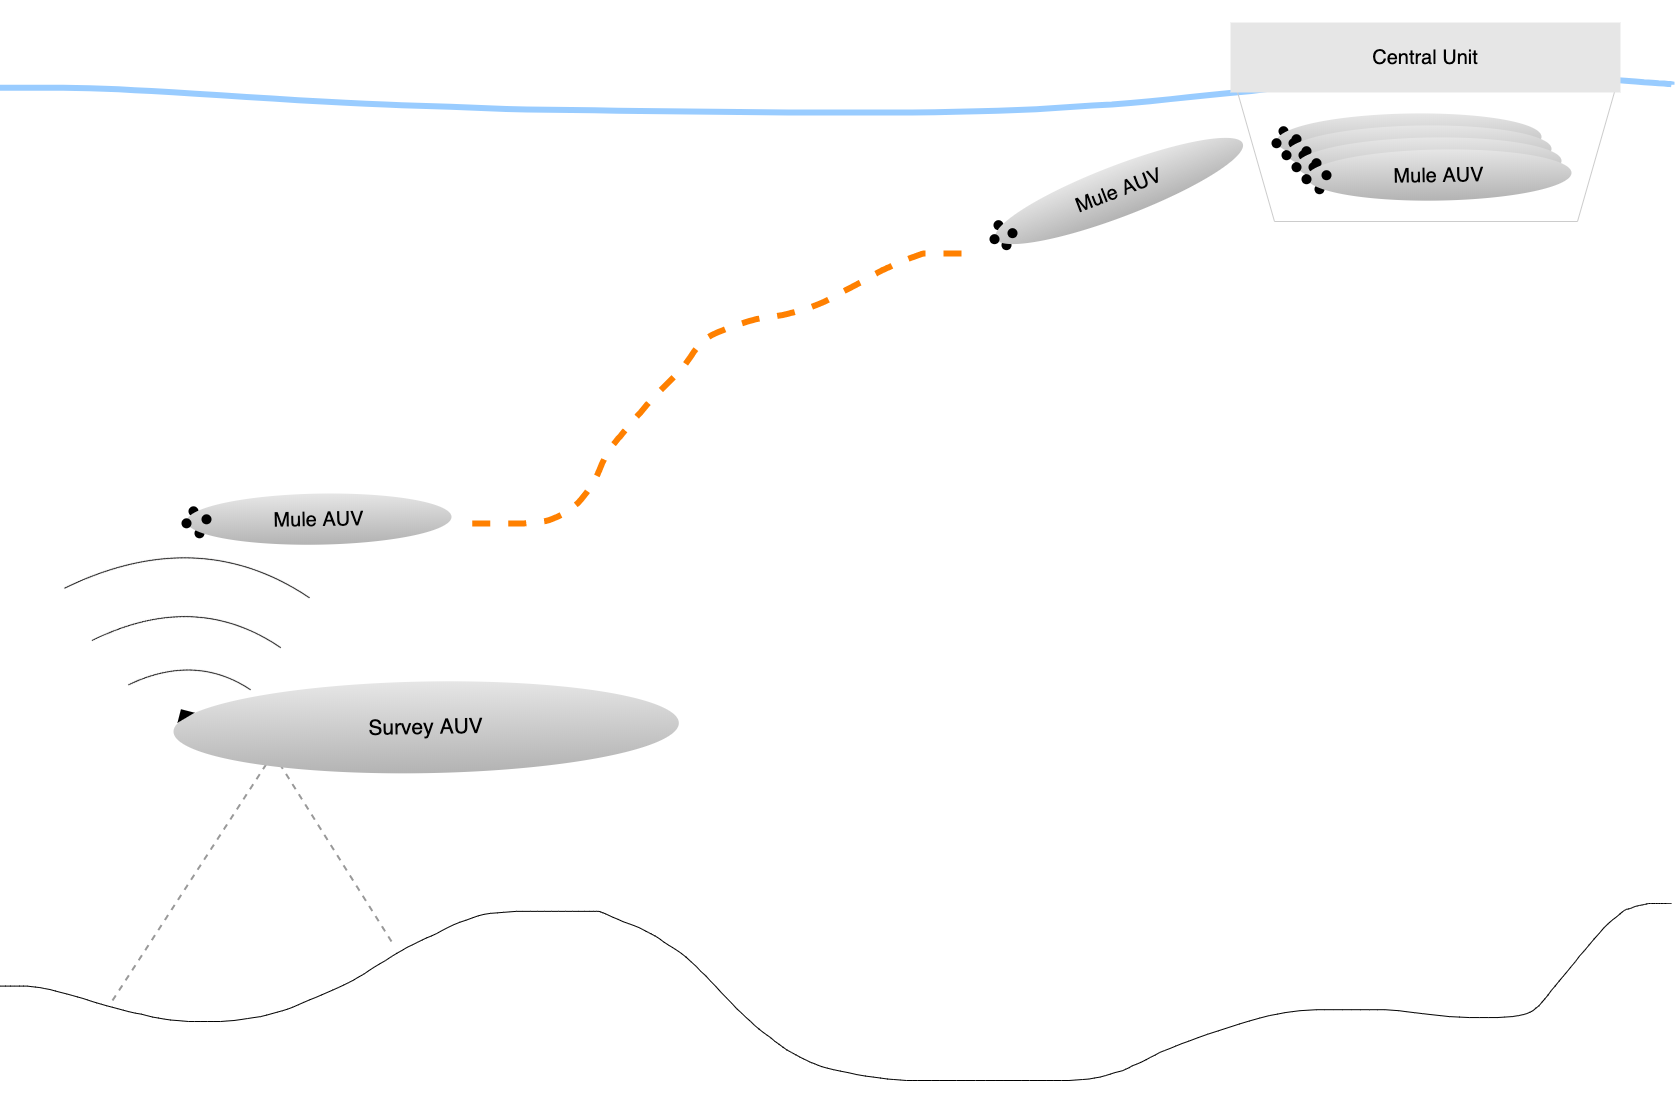
\includegraphics[width=0.9\textwidth]{figures/GROW}
	\caption{Context of the GROW project}
	\label{fig:grow}
\end{figure}

%\begin{figure}[!htbp]
%	\centering
%	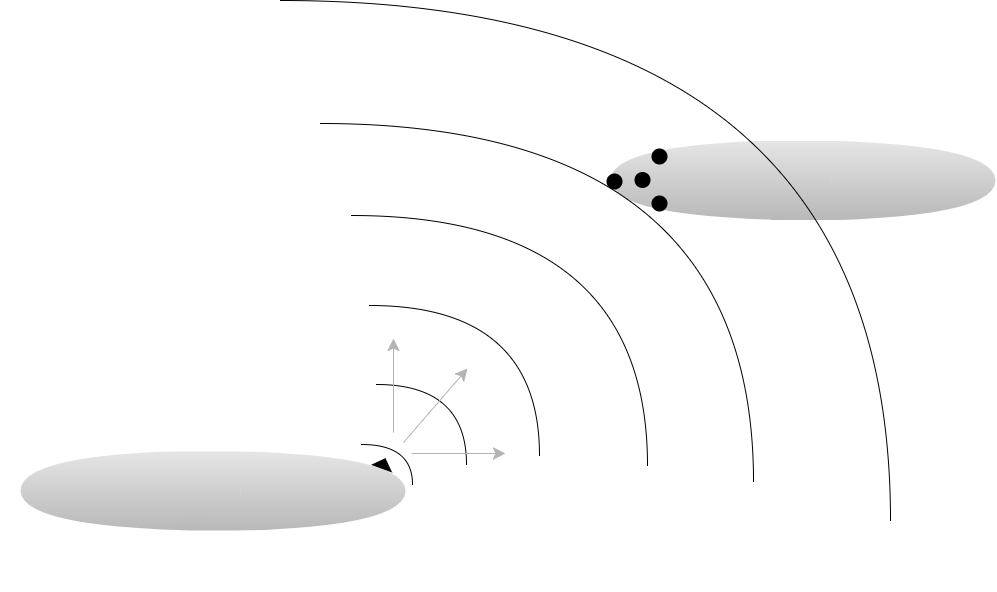
\includegraphics[width=0.8\textwidth]{figures/proposed-solution}
%	\caption{Communication System}
%	\label{fig:auv_scene}
%\end{figure}

This partial USBL system was developed in previous dissertations and research work, which can be better understood in \cite{afonso-thesis}. Briefly, the system consists on a transducer of four hydrophones forming a 3D array deployed on the mule AUV. The distance between AUVs is given by the cross-correlation between the received and expected signals. Since the operation frequency range is around tens of kilohertz, which minimizes the attenuation of sound, the time difference of arrival has to be refined by analyzing the relative phase differences between hydrophones.

Considering that the survey AUV navigates freely trough unknown locations, the USBL system to be employed needs to fulfill particular requirements that common commercial solutions do not comply. 

Firstly, the system needs to be able to cover both short and long range distances, going from tens of centimeters to several hundreds of meters between the receiver and the transmitter, with the best estimation precision possible. For long range positions, the precision of the estimation affects how direct is the path for the mule AUV to reach the acoustic source. This influences the overall energy consumption, duration of navigation search and can affect the reliability of the process. For short range position, an accurate estimate allows to avoid collisions and correctly establish chosen relative positions between vehicles. Additionally, an increase in the frequency of position estimation would consume more power but provide more robust positions, which is desirable for short range scenarios. The available market systems usually offer multiple solutions with different limited operation ranges, which would force to employ more than one system to achieve the mentioned range requirement.

Secondly, the USBL system needs to be capable of detecting incoming signals from any position in space, since the localization detection is solely based on the received signals. Since the system is composed by various sensors, it is expected that they are arranged in varied positions and with different perspectives so they can cover a wider area. However, considering they are supposed to be employed on an AUV, the vehicle's body represents an opaque obstacle to signals. Therefore, with only four fixed hydrophones, it is not possible to detect positions with full line of sight, as intended, since not all hydrophones would have line of sight to the transmitter at all times.

The system that is proposed in this dissertation intended to resolve this technological gap with a system that satisfies the described requirements. Since only four hydrophones are enough to obtain a position estimation (bearing and distance), if they assume a fixed position on an AUV's body it would inevitably limit the direction to where the sensor has direct line of sight. Therefore, the suggested method implies deploying multiple sensors in the vehicle. From the available sensors, only four would be used simultaneously to receive the signals and feed them to the processing system. By adopting this concept, a main issue that arises is where to place the hydrophones within the vehicle. This constitutes the main research topic conducted in the present thesis.

Considering that the mentioned mechanism is meant to be applied in mobile vehicles with changing environment conditions, it is useful to integrate it in a system which is responsive in real time. Accordingly, the process that selects four hydrophones among the available set can be integrated in an adaptive reconfigurable system which enables the hydrophones commutation according to the sensors' configuration that minimizes the estimation error.

The study conducted in the scope of this dissertation intends to prove the functionality of the developed method, validate the hypothesis declared in \ref{sec:hypoth-rq} and draw conclusions on the research questions.

%------------------------------------------------------------------------------------
\section{Assumptions} \label{sec:premises}

This research work relies on a set of premises that were considered throughout the development of the proposed system, as presented in this section.

\paragraph{Number of sensors} For the estimation of the position in 3D space, a multilateration approach was used, as explained in \ref{subsubsec:lateration}. Therefore, a minimum of 4 hydrophones are needed so that it is possible to define the position of the transmitter. Using only two sensors, two possibility spheres are formed around these sensors whose intersection originates a circle that contains the location possible solutions. By adding a third sensor, this circle is intersected by another sphere which originates only two location possibilities. Finally, a fourth sensor is added to exactly differentiate which is the accurate location solution.

\paragraph{Synchronism} The system integrates a synchronization mechanism that allows to know the time of emission of an acoustic signal, hence it is possible to compute the ToA of the signal which indicates the range between the transmitter and the receiver.

\paragraph{Noise characteristics} The system assumes an injected error $e_i$ added to the time differences of arrival, $ \Delta t_{ij}$. These errors are mutually independent and follow a Gaussian distribution with zero mean and a configurable variance of $\sigma^{2}$, i.e., $e_i \sim \mathcal{N}(0,\,\sigma^{2})$. 

For the simulations performed in this project, a deviation of 5$^{\circ}$, or a window of $[-2.5^{\circ},2.5^{\circ}]$, in phase difference estimation of incoming signals was considered to be reasonable for an underwater navigation scenario. This value is based on the observation that the process implemented to calculate the phase difference, using acoustic signals recorded in controlled laboratory environment, produced a stable value within an interval of 2 degrees. Therefore, since the specified period of the signals is $T = \frac{1}{24400}$, then the 5$^{\circ}$ will be equivalent to $\frac{5^{\circ}}{360^{\circ}}*T$ which is approximately a deviation of $0.5\mu s$. Hence the considered standard deviation $\sigma$ to characterize the error $e_i$ in the computed time differences of arrival is equal to $0.5\mu s$.

\paragraph{Reference axis} The origin of the reference axis is defined at the center of the structure where the hydrophones are fixed, which in this case is the AUV.

\paragraph{Propagation speed} The considered speed of sound is 1500 m/s, which corresponds to the underwater propagation velocity of waves in typical conditions.

%------------------------------------------------------------------------------------
\section{Hypothesis and Research Questions} \label{sec:hypoth-rq}

This dissertation intends to complement previous research work and answer to a core research hypothesis which serves as fundamental investigation purpose. This research hypothesis can be stated as:
\\

\textit{"Using a USBL system that reconfigures the hydrophone selection leads to an improvement on the underwater localization precision, allowing to always have a set of four active hydrophones with line of sight to the transmitter and makes it suitable for both short and long range estimation."}
\\

Attending the proposed hypothesis, the topics that are intended to be explored and discussed in this thesis's work can be summarized in the following research questions:

%Research Questions
\begin{description}
	\item[RQ1: ] \textit{What method should be adopted in order to efficiently compare the performance of hydrophone configurations?}
	
	\item[RQ2: ] \textit{What decision metric(s) should be used to evaluate the optimal hydrophone configuration for a specific angle of arrival?}
	
	\item[RQ3: ]\textit{How should the system be developed in order to assure that the selected hydrophones always have line of sight to the transmitter?}
	
	\item[RQ4: ] \textit{Are there distinct best hydrophone configurations for short and long range estimation?}
\end{description}

These questions summarize the main topic points which are explored in the scope of this thesis and are the essential inquiries that it intends to answer.

%------------------------------------------------------------------------------------
\section{Validation Methods} \label{sec:validation}

The validation of scientific work is a key factor to demonstrate how reliable and effective it is. In this thesis, three essential methods are used to validate the functionality of the developed techniques:

\begin{itemize}
	
	\item \textbf{Simulation}
	
	The considered immediate approach to evaluate the functionality and behavior of the system consists in creating a set of simulation procedures which are as close as possible to the real environment and the physical system. These simulations were made as MATLAB scripts carefully designed to integrate realistic parameters, such as expected environment noise and other limitations.
	
	\item \textbf{Scientifically recognized methods}
	
	When composing a system, it can be useful comparing the studied approach with widely used methods which are recognized in the scientific community. By doing this, we can gain a level of confidence in the developed system and in the obtained results.
	
	\item \textbf{Field experiments}
	
	After having the analytical methods and simulations coherent, it is essential then to test the system in a real environment in order to assess the functionality and performances when real conditions are added. By testing it in a real application it is possible to take conclusions about its robustness and consider improvements or refinements for the system.
	Due to the exceptional pandemic situation, in the present work it was only possible to perform field tests on the developed digital signal processing module. 

\end{itemize}
